\subsection{Animieren der aktiven Trips}
\label{sub:animieren_der_aktiven_trips}
  Im Client findet die Visualisierung statt. Er stellt die erste Anfrage an den Server um alle Trips in einem Zeitraum zu bekommen. Die Antwort vom Server ist ein Objekt bestehend aus einer ID und einer \texttt{GeoJSON-FeatureCollection}. Die Verwendung von GeoJSON hat den Vorteil, dass verschiedene Bibliotheken für dieses Format zur Verfügung stehen, die dessen Verarbeitung vereinfacht. Auch Mapbox setzt auf die Verwendung von GeoJSON und ist fest damit verbunden. Der Nachteil von GeoJSON ist seine sehr wortreiche Beschreibung. Dass macht es zwar für Menschen gut lesbar, allerdings auf kosten der Datengröße.

  \begin{algorithm}[H]
    \caption{Animate Vehicle}\label{alg:animate_algorithmus}
    \begin{algorithmic}[1]
        \State ServerQueryTimer $\gets$ 30 Seconds
        \State Vehicles $\gets$ Vehicles Inside Bounding Box
        \State Trips $\gets$ Requested Trips
        \Function{animate}{timestamp}
          \ForAll{Vehicles as Vehicle} \State{
            \If{Vehicle started its Trip} 
              \State \Call{calculateVehiclePosition}{Vehicle}
            \EndIf
            \If{Vehicle not started its Trip}
              \State \Call{checkVehicleActivity}{Vehicle, Trips}
            \EndIf
            \State \Call{checkIfVehicleHasFinished}{Vehicle}
            \State \Call{updateMapWithNewPositions}{Vehicles}
          }\EndFor

          \If{ServerQueryTimer Expired} 
            \State Query Server for New Trips
            \State ServerQueryTimer $\gets$ 30 Seconds
          \EndIf

          \State \Call {animate}{timestamp}
        \EndFunction
    \end{algorithmic}
  \end{algorithm}

  Nachdem die Daten für alle aktiven Trips im Client ankommen, kann für jeden dieser Trips ein Vehicle erstellt werden. In einem Animation-Loop wird für jedes Vehicle pro Frame, eine neue Position berechnet und die Karte wird mit der neuen Position aktualisiert. Algorithmus \ref{alg:animate_algorithmus} beschreibt dies in Pseudo-Code.

  Innerhalb dieses Animation-Loops passieren mehrere Dinge. Zuerst wird geprüft, ob sich ein Vehicle überhaupt im Sichtbereich des Anwenders befindet. Trifft das zu, werden für eben diese Vehicle die Distanzen berechnet und die Position des Vehicles entlang der Polyline interpoliert. Falls das Vehicle seinen Trip noch nicht begonnen hat, wird überprüft, ob dies immer noch der Fall ist. Anschließend werden alle Vehicle geprüft, ob sie ihren Trip bereits beendet haben. Danach wird die Karte mit den neuen Positionen der Vehicle aktualisiert. Während all dies geschieht, läuft ein Timer mit, der nach dem Ablaufen von 30 Sekunden den Server nach neuen Trips abfrägt, womit der Abfragekreislauf von vorn beginnt.

  Das Ergebnis ist die Animation aller Vehicle der momentan aktiven Trips (Abbildung \ref{fig:prozess/animate_all_vehicles}).

  \begin{figure}[htbp]
    \begin{center}
      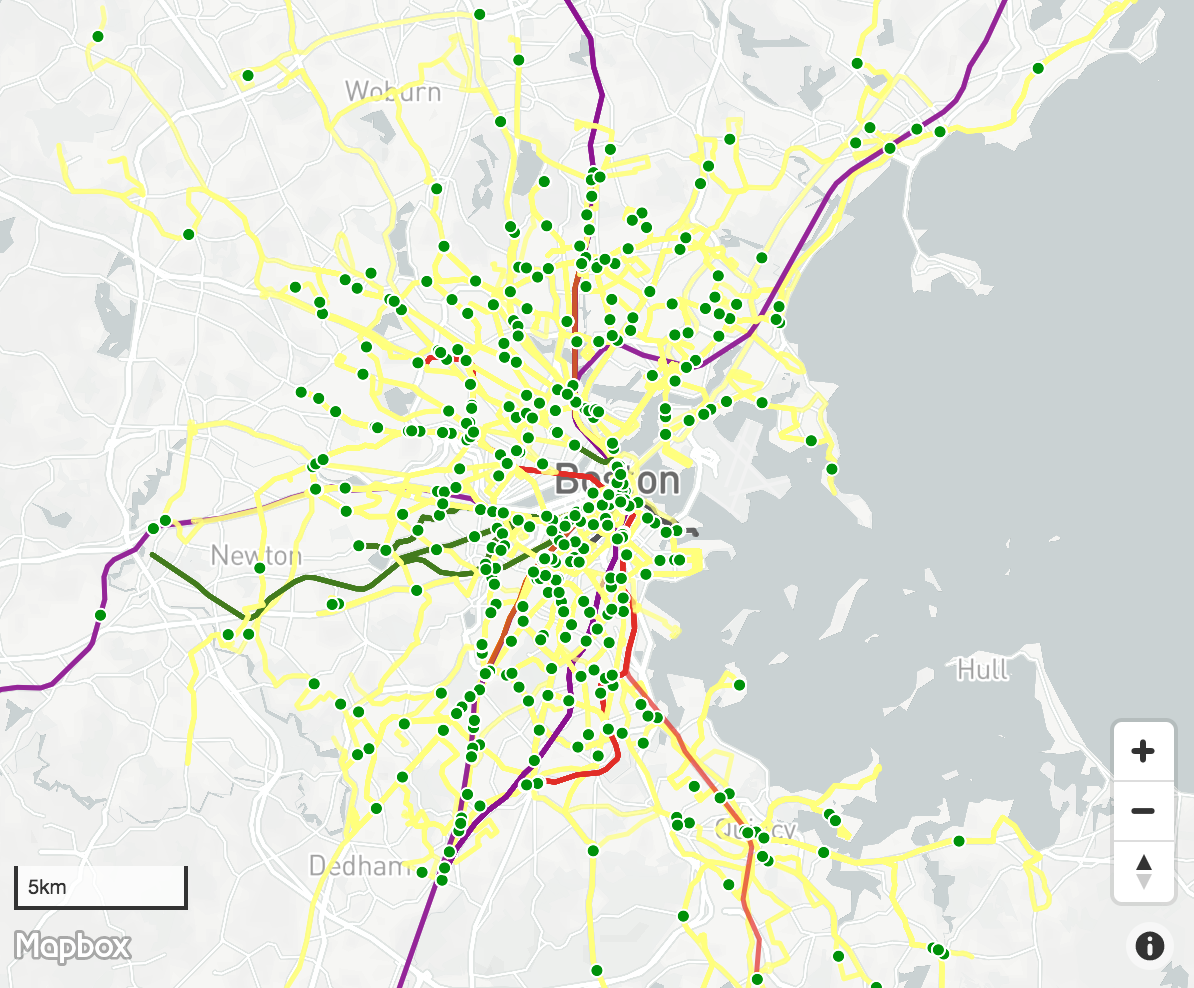
\includegraphics[width=0.7\textwidth]{prozess/animate_all_vehicles}
      \caption{Animieren aller Vehicles auf der Karte}
      \label{fig:prozess/animate_all_vehicles}
    \end{center}
  \end{figure}

  \subsubsection*{Verbesserung der Client Performance}
  \label{ssub:verbesserung_der_client_performance}
    Damit die Animationen auf der Karte bei 60 FPS möglich sind, werden mehrere Optimierungsschritte ausgeführt.

    \begin{itemize}
      \item \textbf{Manipulieren der FPS:} Je niedriger das Zoom Level der Karte, umso geringer wird die FPS eingestellt. Das hat den Hintergrund, dass bei niedrigem Zoom, die Bewegung der Vehicle fast nicht mehr Wahrnehmbar ist. Wohingegen bei höherem Zoom die Animation umso flüssiger sein muss. Folgende Grenzen haben sich bei Tests als gute Werte erwiesen:
      \begin{itemize}
        \item Zoom Level < 12 $\rightarrow$ 1 FPS
        \item Zoom Level > 15 $\rightarrow$ 60 FPS
        \item Sonst $\rightarrow$ 8 FPS
      \end{itemize}
      Dieses Vorgehen bringt den Vorteil, dass bei niedrigem Zoom viel mehr Vehicle angezeigt werden, aber diese nur noch auf 1 FPS animiert werden müssen. Bei hohem Zoom ist dies genau umgekehrt. Dort sind nur noch wenige Vehicle sichtbar, diese werden aber dafür bei 60 FPS animiert. Somit ist einerseits eine gute Performance bei vielen Vehicles möglich und andererseits die Animation bei genauerer Betrachtung trotzdem sehr flüssig.

      \item \textbf{Speichern von Zuständen:} Um Rechenleistung einzusparen, werden wann immer möglich ausgerechnete Werte abgespeichert, damit diese nicht nochmals berechnet werden müssen. Zum Beispiel (siehe Abbildung \ref{fig:polyline_segments}) weiß das Vehicle, auf welchem Polyline Segment\footnotemark es sich befindet. 

       \footnotetext{Ein Segment sei in diesem Kontext ein gerader Linienteil der Polyline, bestehend aus zwei Punkten $A, B$.}

      \begin{figure}[htbp]
        \begin{center}
          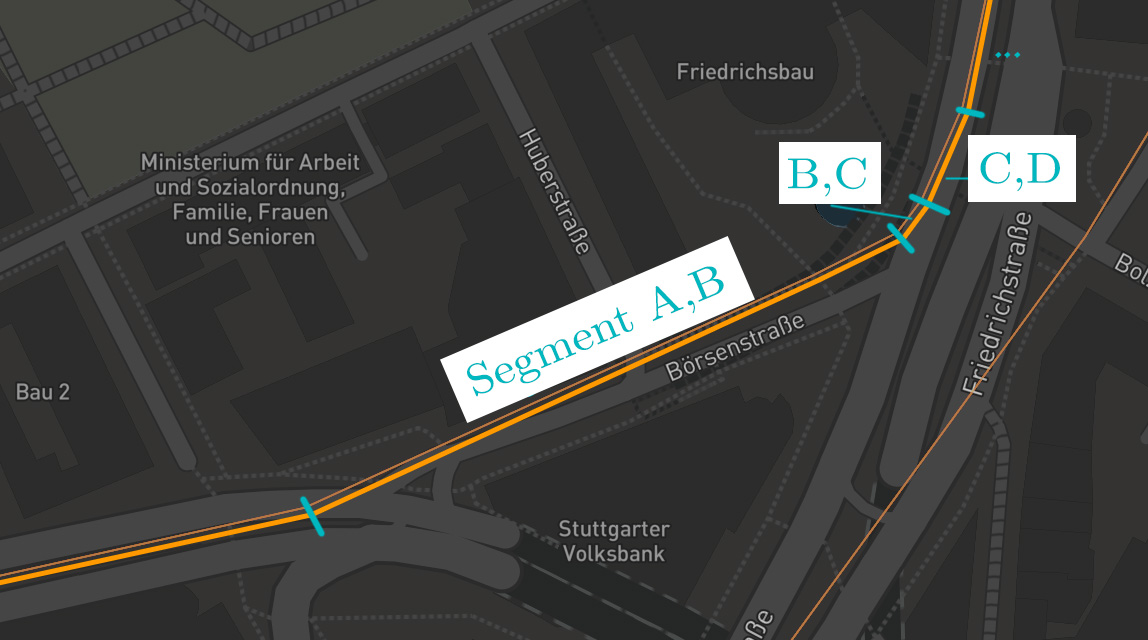
\includegraphics[width=0.6\textwidth]{polyline_segments}
          \caption{Polyline Segmente}
          \label{fig:polyline_segments}
        \end{center}
      \end{figure}

      Das bedeutet, dass die Richtung des Vehicles nicht neu berechnet werden muss, solange es diesem Segment folgt. Erst wenn das Vehicle von Segment $A,B$ auf ein neues Segment $B,C$ übergeht, muss die Richtung neu berechnet werden.

      \item \textbf{Aufteilen der Vehicle in zwei Gruppen:} Da der User durch seinen Bildschirm meistens nur einen Teil der Vehicle zu sehen bekommt, sind die Vehicle in die Gruppen unterteilt. Namentlich seien sie als \texttt{Innerhalb} und \texttt{Außerhalb} benannt. Die Gruppe Innerhalb besitzt all diejenigen Vehicle, die sich im Sichtfeld des Anwenders befinden. Diese werden bei der Animation bevorzugt behandelt und erhalten die volle Rechenleistung. Die Gruppe Außerhalb liegt nicht im Sichtfelds und wird maximal jede Sekunde nach ihrer Aktivität geprüft. Dadurch bleibt auch diese Gruppe immer aktuell.      
    \end{itemize}

    % subsubsection verbesserung_der_client_performance (end)
  
% subsection animieren_der_aktiven_trips (end)